\documentclass[
    11pt, % Set the default font size, options include: 8pt, 9pt, 10pt, 11pt, 12pt, 14pt, 17pt, 20pt
    %
    aspectratio=169, % Uncomment to set the aspect ratio to a 16:9 ratio which matches the aspect ratio of 1080p and 4K screens and projectors
]{beamer}

%\graphicspath{{Images/}{./}} % Specifies where to look for included images (trailing slash required)
\usepackage{booktabs} % Allows the use of \toprule, \midrule and \bottomrule for better rules in tables

%\usepackage{appendixnumberbeamer} %If you want a separate slide counter for your appendix

%%% To add citations
\usepackage[style=authoryear, backend=bibtex]{biblatex}
\addbibresource{references.bib}

%%% Customize Theme %%%%%%%%%%%%%%%%%%%%%%
\usetheme{Madrid} % You can use other themes too, but this changes many things. I've found Madrid to be the best for this color scheme

%fg = font color
%bg = background color

% ! WARNING ! : Many colors are linked to multiple attributes, so changing one color can have unexpected changes!

% If you want to tweak the shading of orange and red, tweak the below 2 lines:t
\definecolor{myGreen}{RGB}{11,102,35}
\definecolor{myOrange}{RGB}{227, 125, 0}

% Bottom right hand color
\setbeamercolor*{structure}{bg=myGreen!20,fg=myGreen!90}

\setbeamercolor*{palette primary}{use=structure,fg=white,bg=structure.fg} %?
\setbeamercolor*{palette secondary}{use=structure,fg=myGreen,bg=white}
    %bottom left of footer & bar between title & top bubbles
\setbeamercolor*{palette tertiary}{use=structure,fg=white,bg=myGreen} 

\setbeamercolor{frametitle}{bg=myGreen!85,fg=white} %title of each slide

\setbeamercolor*{titlelike}{parent=palette primary} %?
%\setbeamercolor{titlelike}{parent=palette primary,fg=structure.fg!50!myRed}

%for miniframe (very top) AND center footer
\setbeamercolor{section in head/foot}{fg=myOrange, bg=white}

%%% Specific Colors %%%
\setbeamercolor{item projected}{bg=myOrange}
\setbeamertemplate{enumerate items}{bg=myOrange}

\setbeamercolor{itemize item}{fg=myOrange}
\setbeamercolor{itemize subitem}{fg=myOrange}

\setbeamercolor{button}{bg=myOrange}

%%% Edits ONLY the TOC slide %%%
\setbeamercolor{section in toc}{fg=black}
\setbeamercolor{subsection in toc}{fg=black}

%%% Block Colors %%%
% Standard block %
    \setbeamercolor{block title}{bg=myOrange, fg=white}
    \setbeamercolor{block body}{bg=myOrange!20}

% Alerted block % If you want to customize it's color
    %\setbeamercolor{block title alerted}{bg=cyan, fg=white}
    %\setbeamercolor{block body alerted}{bg=cyan!10}

% Example block % If you want to customize it's color
    %\setbeamercolor{block title example}{bg=cyan, fg=white}
    %\setbeamercolor{block body example}{bg=cyan!10}

%---------------------------------------------------------
%	SELECT FONT THEME & FONTS
%---------------------------------------------------------
\usefonttheme{default} % Typeset using the default sans serif font
\usepackage{palatino} % Use the Palatino font for serif text
\usepackage[default]{opensans} % Use the Open Sans font for sans serif text
\useinnertheme{circles}

%---------------------------------------------------------
%	SELECT OUTER THEME
%---------------------------------------------------------
% Outer themes change the overall layout of slides, such as: header and footer lines, sidebars and slide titles. Uncomment each theme in turn to see what changes it makes to your presentation.

%\useoutertheme{default}
%
\useoutertheme{miniframes}
\setbeamertemplate{headline}{}

%\useoutertheme{infolines}
%\useoutertheme{smoothbars}
%\useoutertheme{sidebar}
%\useoutertheme{split}
%\useoutertheme{shadow}
%\useoutertheme{tree}
%\useoutertheme{smoothtree}

%---------------------------------------------------------
%	PRESENTATION INFORMATION
%---------------------------------------------------------

\title[]{Autonomous Mobile Robotics}
\subtitle[]{Ray Casting \& Ray tracing}
\author[]{Author: Igor Alentev}

\institute[]{Innopolis University \\ \smallskip \textit{i.alentev@innopolis.university}}
\date[IU S23]
%\date[\today]

\logo{}

%---------------------------------------------------------
%---------------------------------------------------------
%---------------------------------------------------------
\begin{document}

%---------------------------------------------------------
%	TITLE SLIDE
%---------------------------------------------------------
\section{}
\begin{frame}
	\titlepage % Output the title slide, automatically created using the text entered in the PRESENTATION INFORMATION block above
 
\end{frame}

%---------------------------------------------------------
%	TABLE OF CONTENTS SLIDE
%---------------------------------------------------------
% References sections and subsections, specified with the standard \section and \subsection commands. If you want to display all sections and subsections on one slide, just use \tableofcontents. If you want to just display each section one at a time (in subsequent slides) use \tableofcontents[pausesections].

\begin{frame}
	\frametitle{Table of Contents} % Slide title, remove this command for no title
	
	\tableofcontents % Output the table of contents (all sections on one slide)
	%\tableofcontents[pausesections] % Output the table of contents (break sections up across separate slides)
\end{frame}

%---------------------------------------------------------
%	PRESENTATION BODY SLIDES
%---------------------------------------------------------

\section{Introduction to RC \& RT}

\begin{frame}
    \frametitle{Ray casting \& Ray tracing}
    \begin{columns}[c]
        \begin{column}{0.5\textwidth}
            \begin{itemize}
                \item What is a ray?
                \item What are those ray techniques?
                \item What are the differences between them?
                \item Are they actually used in robotics?
            \end{itemize}
        \end{column}
        \begin{column}{0.5\textwidth}
            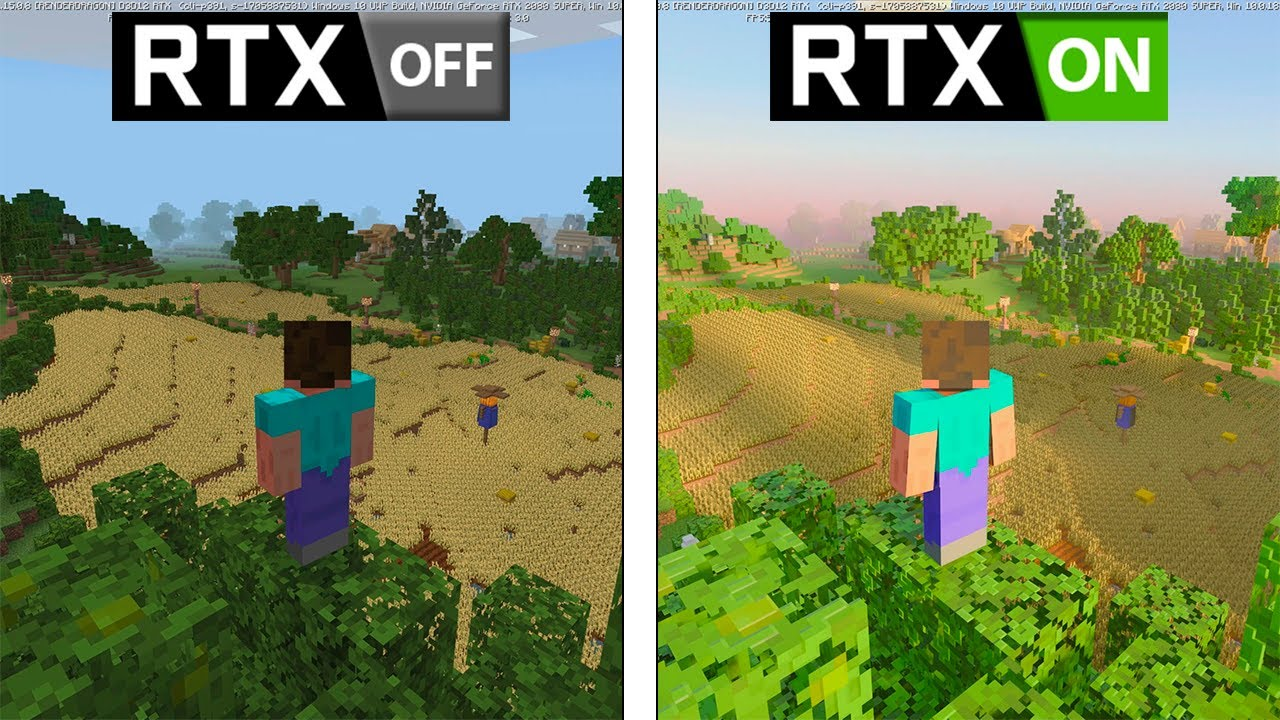
\includegraphics[scale=0.16]{assets/minecraftrtx.jpg}
        \end{column}
    \end{columns}
    
\end{frame}

\begin{frame}
    \frametitle{Ray casting \& Ray tracing}
    \begin{itemize}
        \item Not necesasrily a light ray. For instance, sound-ray approaches to ray tracing.
        \item Ray tracing and ray casting are methods of building
              the scene based on the intersection of rays with scene objects.
        \item Ray casting is easy and simple algorithm only searching for one intersection. Ray tracing algorithms
              are capable of recursively tracing reflexions. Both algorithms used to visualize an object calculating a color
              of each pixel during projection on the camera plane.
        \item They are both used in robotics in various ways.
    \end{itemize}
\end{frame}

\begin{frame}
    \frametitle{Ray casting \& Ray tracing}
    \begin{columns}[c]
        \begin{column}{0.5\textwidth}
            \begin{center}
                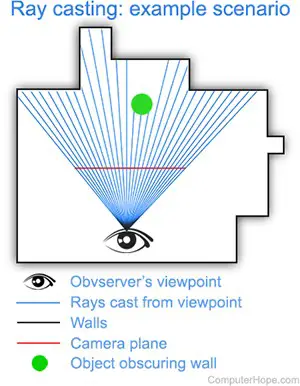
\includegraphics[scale=0.5]{assets/ray-casting-diagram.jpg}
            \end{center}
        \end{column}
        \begin{column}{0.5\textwidth}
            \begin{center}
                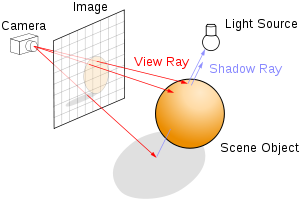
\includegraphics[scale=0.6]{assets/300px-Ray_trace_diagram.svg.png}
            \end{center}
        \end{column}
    \end{columns}
\end{frame}

\section{Global Path Planning}

\subsection{Ray Casting and Tracking}

\begin{frame}
    \frametitle{Ray casting and Tracking\footcite{kimSimpleGlobalPath2018}}
    \begin{columns}[c]
        \begin{column}{0.5\textwidth}
            Having global path planning problem one can use ray casting as an efficient way of finding a most optimal path.
            \newline\newline
            However, this path does not seem optimal enough?
        \end{column}
        \begin{column}{0.5\textwidth}
            \begin{figure}
                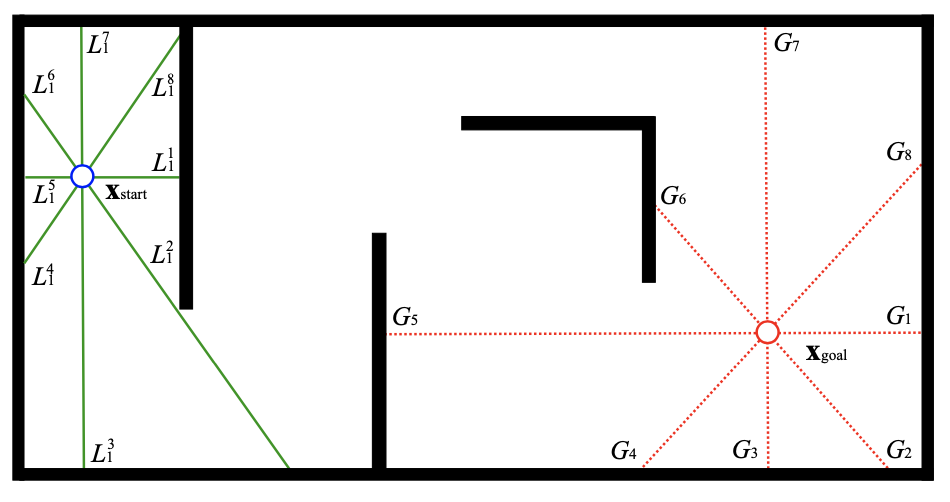
\includegraphics[scale=0.23]{assets/rct-init.png}
                \caption{Initialization}
            \end{figure}
            \begin{figure}
                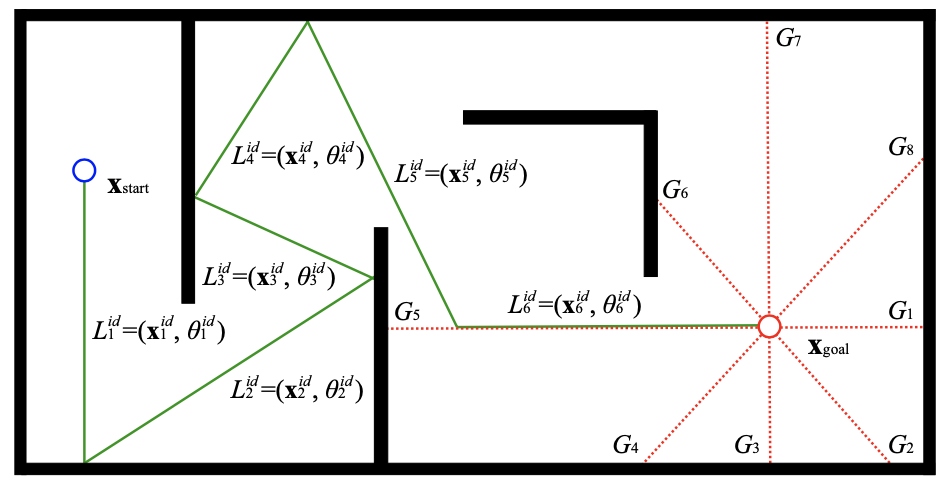
\includegraphics[scale=0.23]{assets/rct-expand.png}
                \caption{Expansion}
            \end{figure}
        \end{column}
    \end{columns}
\end{frame}

\begin{frame}
    \frametitle{Ray casting and Tracking}

    \begin{columns}[c]
        \begin{column}{0.5\textwidth}
            That is why we need one more algorithm step --- trimming.
            \newline\newline
            And finally trimming interpolation.
        \end{column}
        \begin{column}{0.5\textwidth}
            \begin{figure}
                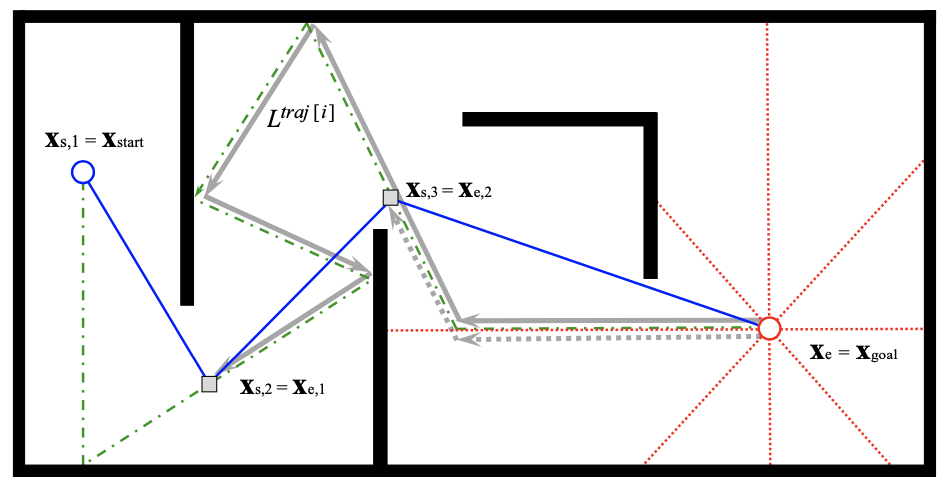
\includegraphics[scale=0.23]{assets/rct-trimming.png}
                \caption{Trimming}
            \end{figure}
            \begin{figure}
                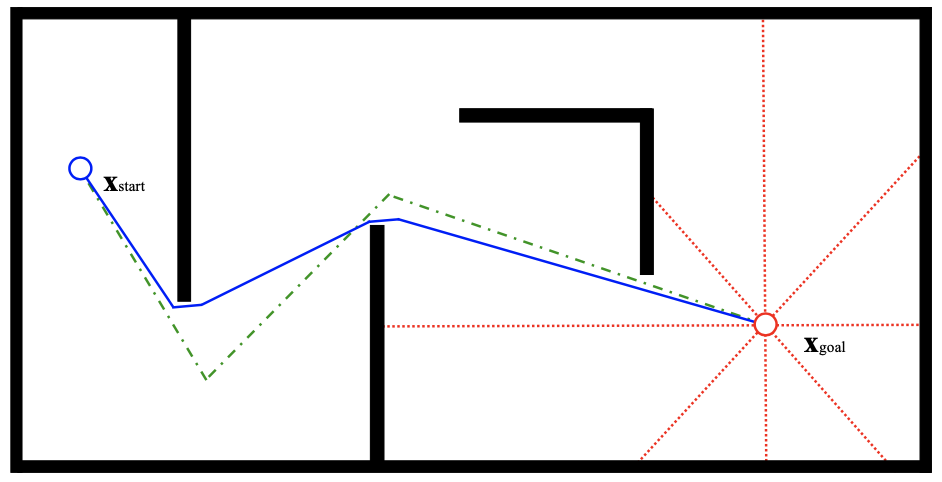
\includegraphics[scale=0.23]{assets/rct-int-trimming.png}
                \caption{Trimming interpolation}
            \end{figure}
        \end{column}
    \end{columns}

\end{frame}

\begin{frame}
    \frametitle{Ray casting and Tracking}

    \begin{columns}
        \begin{column}{0.5\textwidth}
            \begin{figure}
                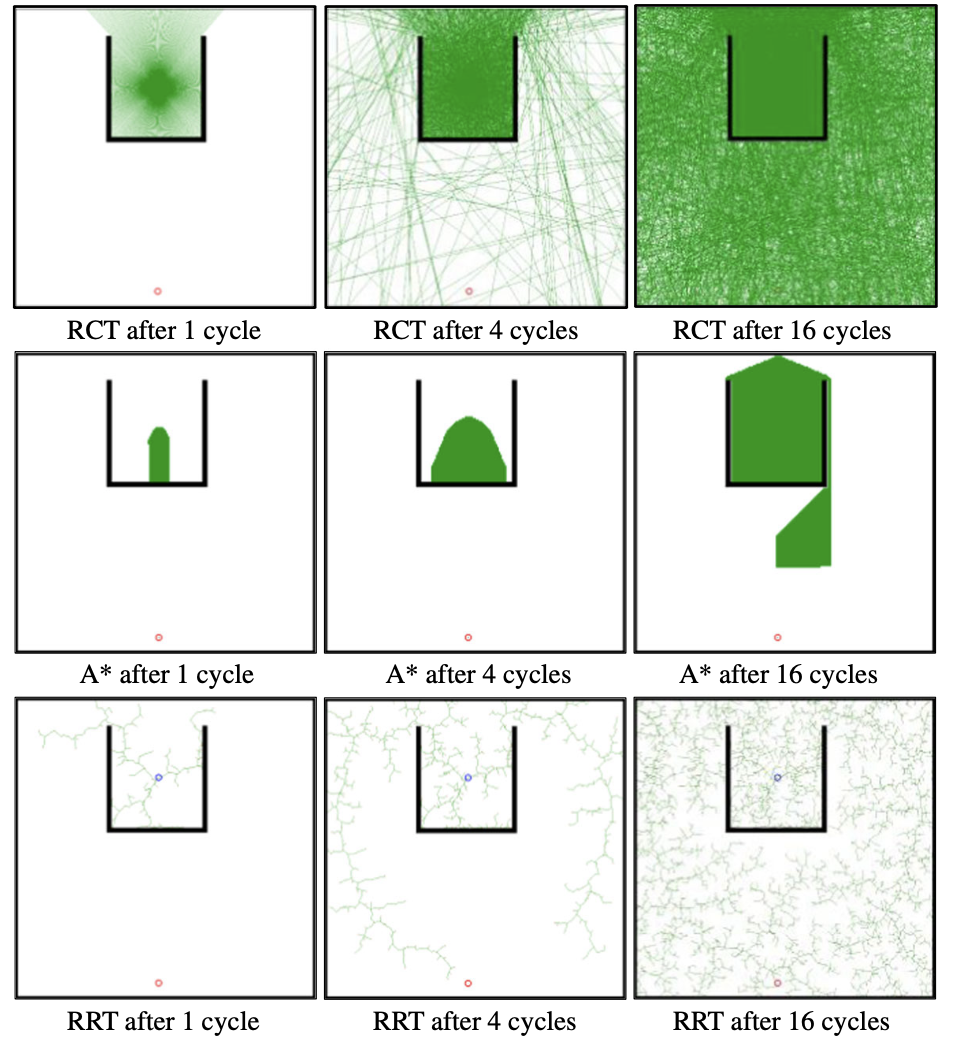
\includegraphics[scale=0.3]{assets/rct-conv-comparison.png}
                \caption{Comparison of $RCT$, $A^*$ and $RRT$}
            \end{figure}
        \end{column}
        \begin{column}{0.5\textwidth}
            \begin{figure}
                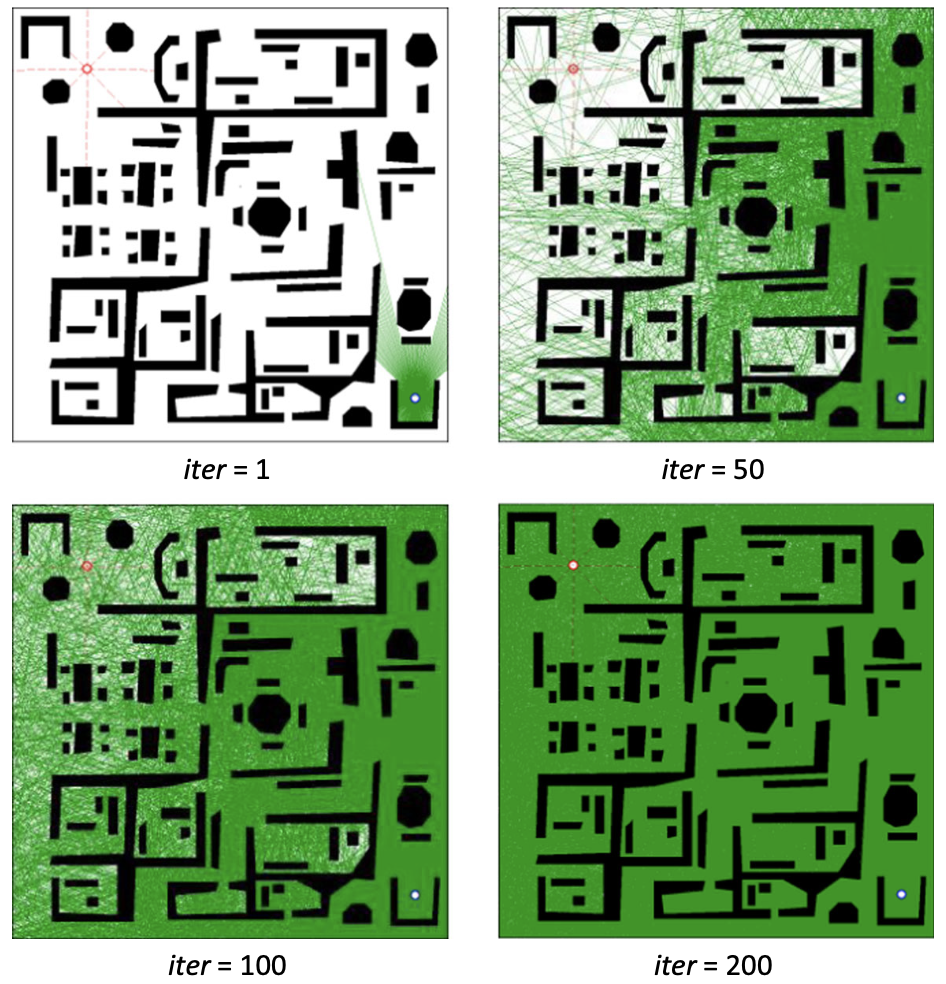
\includegraphics[scale=0.3]{assets/rct-example.png}
                \caption{RCT in action example}
            \end{figure}
        \end{column}
    \end{columns}

\end{frame}

\section{Local Path Planning}

\subsection{Colision Avoidance in Sailing Robots}

\begin{frame}
    \frametitle{Collision Avoidance in Sailing Robots\footcite{sauzeRaycastApproachCollision2010}}

    \begin{columns}[c]
        \begin{column}{0.5\textwidth}
            Sailing robots typically equipped with a small embedded computer require computationally efficient, simple
            and at the same time comprehensive solution to collision avoidance.
        \end{column}
        \begin{column}{0.5\textwidth}
            \begin{center}
                \begin{figure}
                    \caption{Ray casting example}
                    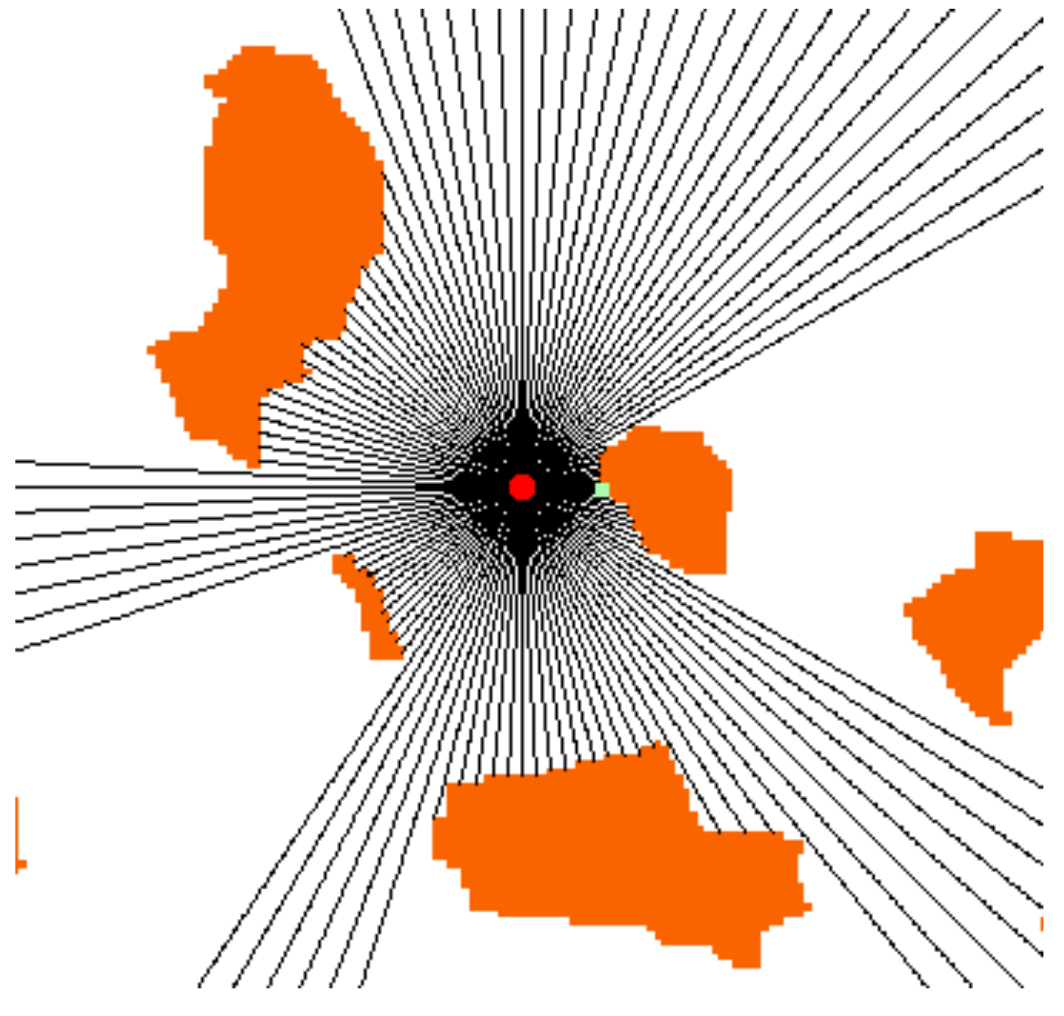
\includegraphics[scale=0.25]{assets/casr-raycast-example.png}
                \end{figure}
            \end{center}
        \end{column}
    \end{columns}
\end{frame}

\begin{frame}
    \frametitle{Collision Avoidance in Sailing Robots}

    \begin{columns}[c]
        \begin{column}{0.5\textwidth}
            We should consider:
            \begin{itemize}
                \item Coastline data
                \item Ship locations
                \item Weather information
                \item Other hazards
            \end{itemize}
        \end{column}
        \begin{column}{0.5\textwidth}
            \begin{center}
                \begin{figure}
                    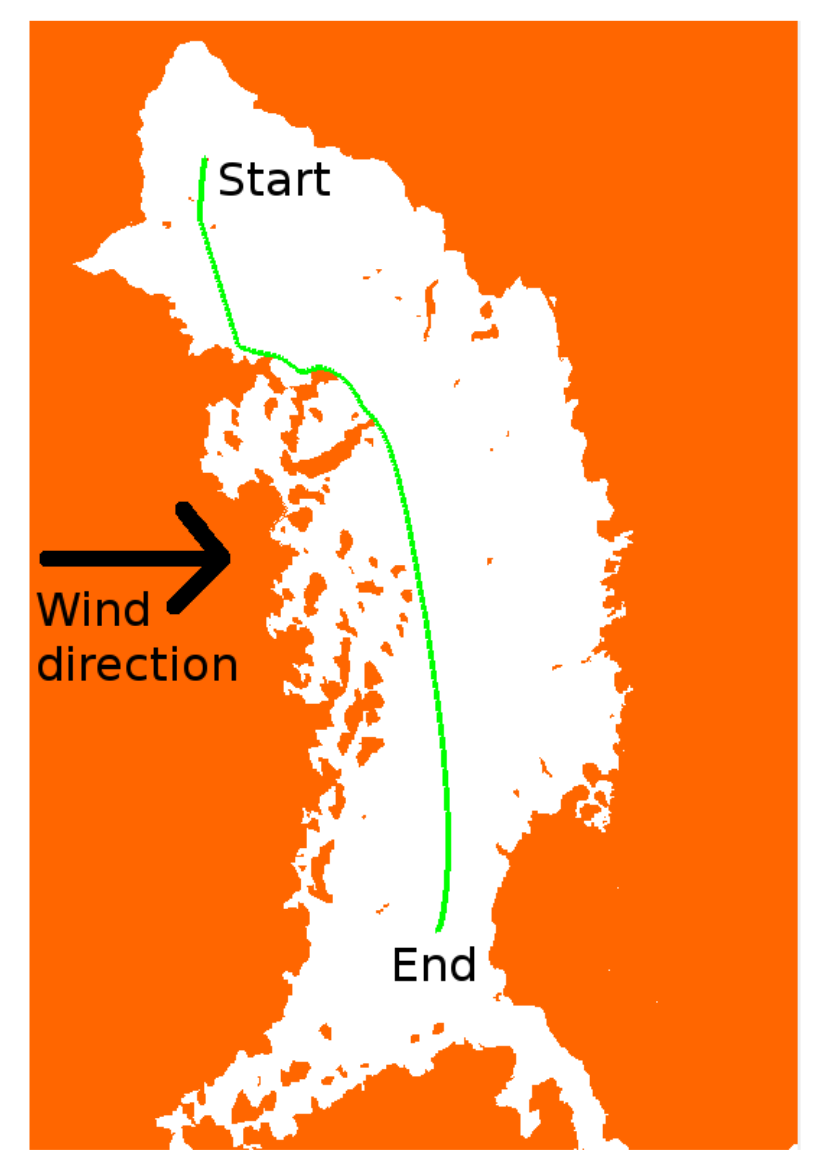
\includegraphics[scale=0.25]{assets/casr-result.png}
                    \caption{The course sailed by the robot in Strangford Lough.}
                \end{figure}
            \end{center}
        \end{column}
    \end{columns}
\end{frame}

\begin{frame}
    \frametitle{Collision Avoidance in Sailing Robots}

    \begin{columns}[c]
        \begin{column}{0.5\textwidth}
            \begin{itemize}
                \item We can vary scanning angle
                \begin{itemize}
                    \item Too wide angle more computationally heavy and makes
                    it difficult to analyse obstacles on heading direction.
                    \item Too narrow angle ignores obstacles which we may face after
                    changing heading direction
                \end{itemize}
                \item It seems that optimal path is the closest free beam to the target (more on that in original paper)
            \end{itemize}
        \end{column}
        \begin{column}{0.5\textwidth}
            \begin{figure}
                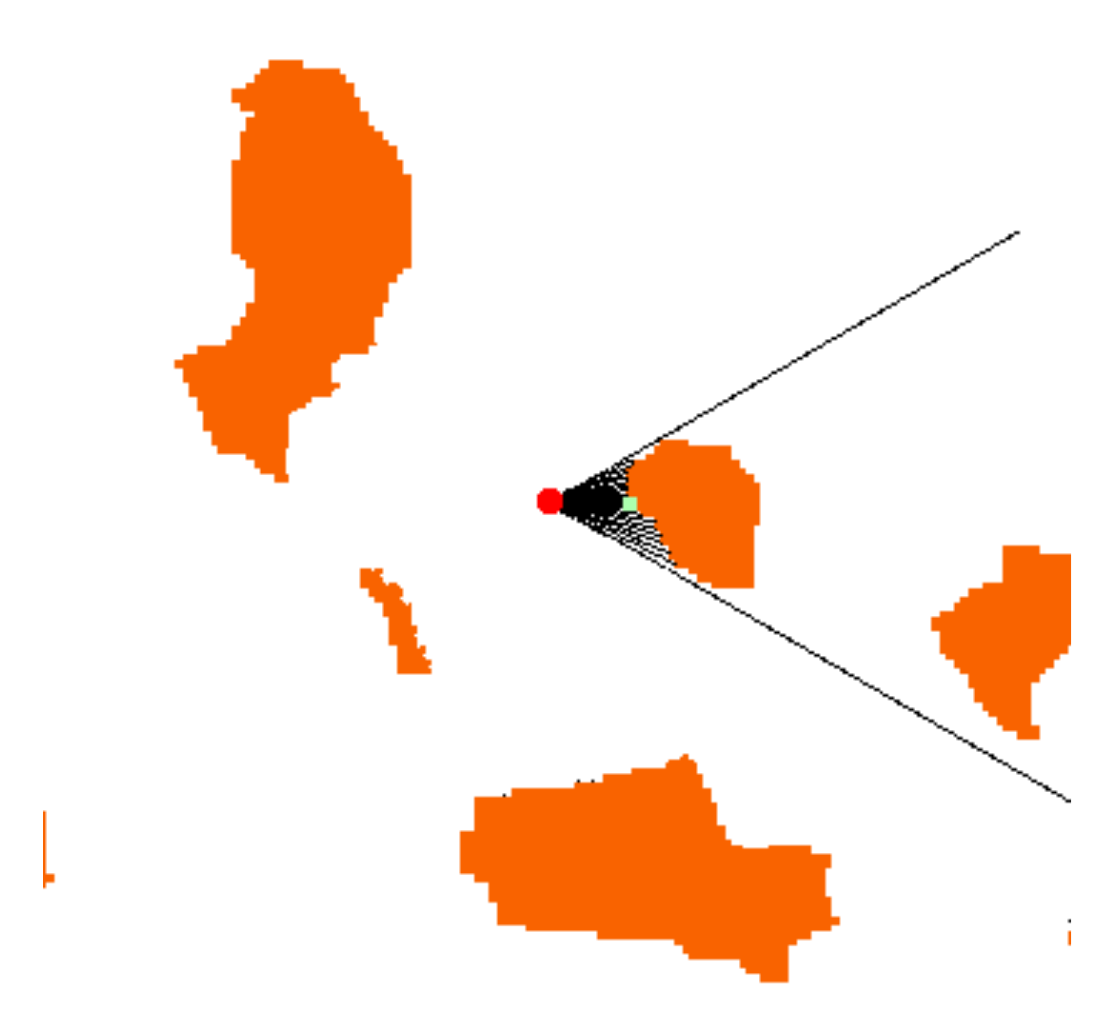
\includegraphics[scale=0.25]{assets/casr-angle-example.png}
                \caption{60 degree wide beam.}
            \end{figure}
        \end{column}
    \end{columns}
\end{frame}

\section{Localisation}

\subsection{Real-time Ray-tracing}

\begin{frame}
    \frametitle{RT2 --- Real-time ray-tracing\footcite{casalinoRTRealtimeRaytracing2011}}

    Imagine having a fleet of AUVs (Autonomous Underwater Vehicles) each equipped with on-board acoustic modem.
    How to localize them?

    \begin{columns}[t]
        \begin{column}{0.5\textwidth}
            Acoustic localization:
            \begin{itemize}
                \item Several vehicles are on the surface and GPS-linked
                \item Underwater vehicles build a localization net
                \item Acoustic localization algorithms allow to localize a vehicle
                      w.r.t.\ other vehicles, for instance, GPS-linked.
            \end{itemize}
        \end{column}
        \begin{column}{0.5\textwidth}
            \begin{center}
                \begin{figure}
                    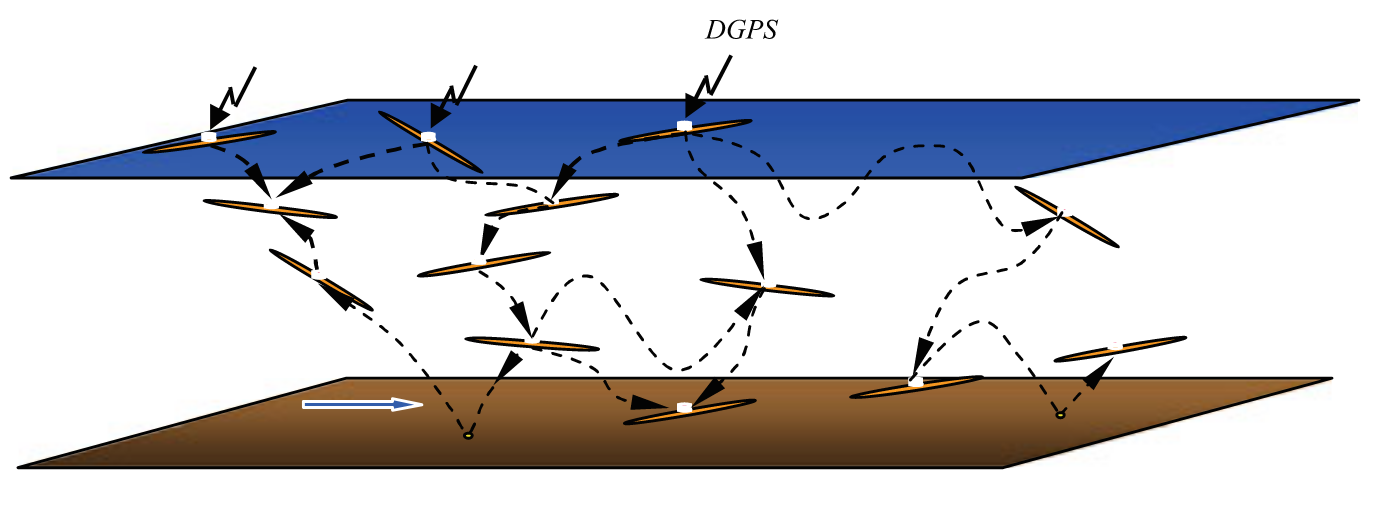
\includegraphics[scale=0.3]{assets/rt2-localization.png}
                    \caption{Acoustic localization concept}
                \end{figure}
                
            \end{center}
        \end{column}
    \end{columns}
\end{frame}

\begin{frame}
    \frametitle{RT2 --- Real-time ray-tracing}
    \begin{itemize}
        \item Assuming we know sound velocity profile as the function of depth a-priori, we 
        can build look-up tables and sound-rays tracing in such a way that units will
        be able to localize themselves.
        \item Simulation show that perfectly knowing sound profile allows us to have
        an accuracy with errors of around few centemeters. Moreover, even under
        uncertainties algorithm has proven working well.
    \end{itemize}
\end{frame}

\section{Others}

\subsection{Coverage Path Planning}

\begin{frame}
    \frametitle{Coverage Path Planning\footcite{felsnerRoboticCoveragePath2021}}

    \begin{columns}[c]
        \begin{column}{0.5\textwidth}
            Having region of interest which should be inspected, we can use ray tracing to 
            generate volumetric representation of the covered regions. 
            \newline\newline
            Moreover, ray tracing is done via the ultrasonic testing of the environment.
        \end{column}
        \begin{column}{0.5\textwidth}
            \begin{figure}
                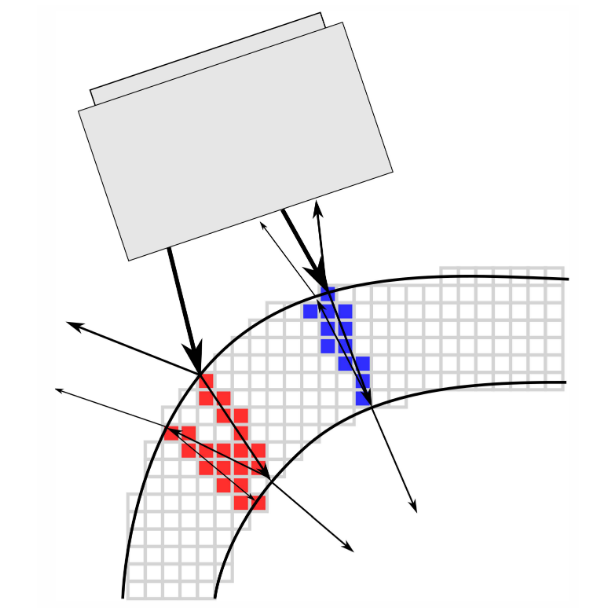
\includegraphics[scale=0.4]{assets/cpp-example.png}
                \caption{UT example}
            \end{figure}
        \end{column}
    \end{columns}

    

\end{frame}

\subsection{Audio Ray-Tracing}

\begin{frame}
    \frametitle{Audio position estimation\footcite{evenAudioRayTracing2014}}

    A robot can detect objects in the blind region of its laser range if those objects emit sound.
    \newline\newline
    Having information about acoustic reflection and estimated via ray tracing directions of arrival 
    of the sound we can detect objects that are not visible, but can be heard.

\end{frame}

% \section{Motivation} % Note all sections and subsections are automatically placed in your table of contents

% %------------------------------------------------
% \begin{frame}
% 	\frametitle{Title}
%             \begin{center}
%                 \textbf{To use this template, you can copy and just edit/add slides!}\newline   
%             \end{center}
            
%             This is because all of the color customization occurs in the "Customize Themes" section in lines 12-51 of the code\newline

%             The remainder of these slides serve as an example to show all the features you can use: bullets, buttons, sections, etc.

%             \begin{center}
%                 \emph{This was a labor of love, I hope you like it!}
%             \end{center}
% \end{frame}

% %------------------------------------------------
% \begin{frame}
% 	\frametitle{Another Title}
% 	\framesubtitle{and a subtitle!}
	
% 	Look at the code of this slide to see how columns made this formatting look nice.

% 	\begin{columns}[t] % The "c" option specifies centered vertical alignment while the "t" option is used for top vertical alignment
% 		\begin{column}{0.5\textwidth} % Right column width
%                 % To add an image %
%                 \begin{figure}[h!] 
%                     \centering
%                     %\caption{Hawkins et al, 2015}
%                     \includegraphics[angle=0, width=4.5cm]{Hokie2.png}
%                     %\label{Figure 1}
%                 \end{figure}
% 		\end{column}
%   		\begin{column}{0.5\textwidth} % Left column width
%                 \begin{figure}[h!]
%                     \centering
%                     %\caption{Hawkins et al, 2015}
%                     \includegraphics[angle=0, width=4.5cm]{Hokie2.png}
%                     %\label{Figure 1}
%                 \end{figure}
% 		\end{column}		
% 	\end{columns}
% \end{frame}

% %------------------------------------------------
% \begin{frame}
% 	\frametitle{Yet another title}
%             You can use bullets too:\newline
%             \begin{itemize}
%                 \item Like this one\newline
%                 \item \& this one
%             \end{itemize}
% \end{frame}

% %------------------------------------------------
% \begin{frame}
% \label{Test} %For the link button for the Appendix slide
% 	\frametitle{A title}

%         \begin{itemize}
%             \item You can also nest sub-bullets
%             \begin{itemize}
%                 \item Sub-bullet 1
%                 \item Sub-bullet 2
%                 \item Sub-bullet 3
%                 \item Sub-bullet 4 \newline
%             \end{itemize}
%         \end{itemize}

%         You can add citations \footcite{casalinoRTRealtimeRaytracing2011} too\newline

%         \textbf{Below is a button that links to a slide in the appendix}
        
%         \begin{center}
%             \hyperlink{Figure}{\beamergotobutton{Go to graphs}}    
%         \end{center}
% \end{frame}

% %------------------------------------------------
% \section{Theory}

% %------------------------------------------------
% \begin{frame}
% \label{Test Stat}
% 	\frametitle{The Test Statistic}
		
%         Here is a made up equation:
%         $$ \hat{A} = \bar{m}-\hat{m}_S$$ \newline

%         Notice how these buttons are centered and evenly spread out:\newline

%         \begin{columns}[t] % The "c" option specifies centered vertical alignment while the "t" option is used for top vertical alignment
% 		\begin{column}{0.25\textwidth} % Right column width
%                 \hyperlink{Terms}{\beamergotobutton{Go to Terms}}
% 		\end{column}
%   		\begin{column}{0.25\textwidth} % Left column width
%                 \hyperlink{Definitions}{\beamergotobutton{Go to Definitions}}
% 		\end{column}
%             \begin{column}{0.25\textwidth} % Left column width
%                 \hyperlink{Theorems}{\beamergotobutton{Go to Theorems}}
% 		\end{column}
% 	\end{columns}
        
% \end{frame}

% %------------------------------------------------
% \begin{frame}
% 	\frametitle{No way, another title!}
%             \begin{enumerate}
%                 \item Instead of bullets, you can index by number too\newline
%                 \item like this
%             \end{enumerate}
% \end{frame}

% %------------------------------------------------
% \section{Testing}

% %------------------------------------------------
% \begin{frame}
% 	\frametitle{Second to last title}
%     	\begin{block}{Block Title}
%     		Block 1
%     	\end{block}
    	
%     	\begin{exampleblock}{Example Block Title}
%     		Block 2
%     	\end{exampleblock}
    	
%     	\begin{alertblock}{Alert Block Title}
%     		Block 3
%     	\end{alertblock}
    	
%     	\begin{block}{} % Block without title
%     		Block without a title
%     	\end{block}
% \end{frame}

% %------------------------------------------------
% \section{Conclusion}
% %------------------------------------------------
% \begin{frame}
% 	\frametitle{Last title}
		
% 	Last bit of text

% \end{frame}

% %---------------------------------------------------------
% %	CLOSING SLIDE
% %---------------------------------------------------------

% % To remove miniframe from top
% \appendix
% \setbeamertemplate{headline}{}
% \addtobeamertemplate{frametitle}{\vspace*{-\headheight}}{}

% \begin{frame}[noframenumbering] %So the end and appendix slides don't contribute to the page count
% %[plain] % The optional argument 'plain' hides the headline and footline
% 	%\frametitle{Questions?}

% 	\begin{center}
%             {\LARGE Questions?}
% 	\end{center}
 
% \end{frame}

%---------------------------------------------------------
%	REFERENCES
%---------------------------------------------------------

\begin{frame}[noframenumbering, allowframebreaks] 
        \frametitle{References}

        \printbibliography
\end{frame}

%------------------------------------------------
% \begin{frame}[noframenumbering]
% \label{Figure}
% 	\frametitle{Appendix - A figure}
%         \hyperlink{Test}{\beamerreturnbutton{Return to presentation}}
        
%         \begin{figure}[h!]
%             \centering
%             %\caption{}
%             \includegraphics[angle=0, width=5cm]{Newey et al Graph.png}
%             %\label{fig}
%         \end{figure}
% \end{frame}

% %------------------------------------------------
% \begin{frame}[noframenumbering]
% \label{Terms}
% 	\frametitle{Appendix - Terms}

%         \begin{columns}[t] % The "c" option specifies centered vertical alignment while the "t" option is used for top vertical alignment
% 		\begin{column}{0.5\textwidth} % Right column width
%                 Some Estimators:
%                 \begin{itemize}
%                     \item Drift: $\hat{\delta}$
%                     \item Boundary: $\hat{b}(t)$
%                 \end{itemize}
% 		\end{column}
%   		\begin{column}{0.5\textwidth} % Left column width
%                 Some Variables:
%                 \begin{itemize}
%                     \item $\hat{V}$
%                     \item $\hat{m}_S$
%                     \item $\bar{m}$
%                     \item $m_J(\tau)$\newline\newline
%                 \end{itemize}
% 		\end{column}
% 	\end{columns}
%         \hyperlink{Test Stat}{\beamerreturnbutton{Return to presentation}}        
% \end{frame}

% %------------------------------------------------
% \begin{frame}[noframenumbering]
% \label{Definitions}
% 	\frametitle{Appendix - Definitions}
%          \begin{enumerate}
%              \item A definition \newline
%          \end{enumerate}
         
%         \hyperlink{Test Stat}{\beamerreturnbutton{Return to presentation}}
% \end{frame}

% %------------------------------------------------
% \begin{frame}[noframenumbering]
% \label{Theorems}
% 	\frametitle{Appendix - Theorems}
%          \begin{enumerate}
%              \item A theorem\newline
%          \end{enumerate}
         
%         \hyperlink{Test Stat}{\beamerreturnbutton{Return to presentation}}        
% \end{frame}

\end{document} 